\documentclass[10pt,a4paper,final]{article}
\usepackage[utf8]{inputenc}
\usepackage{amsmath}
\usepackage{tcolorbox} 
\usepackage{float}
\usepackage{amsfonts}
\usepackage{amssymb}
\usepackage{graphicx}
\usepackage[export]{adjustbox}
\tcbuselibrary{breakable}
\newtheorem{thm}{Theorem}
\newtheorem{defn}[thm]{Definition} 
\newtheorem{exmp}[thm]{Example} % same for example numbers

\title{Triangulation Survey Simulation\\\vspace{0.2in} \emph{Preliminary Results}}
\author{Stuart Burrell}

%\graphicspath{home/Dropbox/academic/phd/gibbons/gibbon_simulation/plots}

\begin{document}
\newcommand{\Int}{\int\limits}

\maketitle

\section{Introduction}
The purpose of this short report is to document the method and preliminary results of a triangulation survey simulation. This was motivated by discrepancies with spatial capture-recapture methods. Moreover, the results presented are controversial, and thus, given the early stage of this work, feedback to improve  validity would be greatly appreciated\footnote{sb235@st-andrews.ac.uk}.

\section{Methodology}

The literature on triangulation surveys has some variability, and so we begin
by describing the exact version of the method, from \cite{tri}, that we have investigated. Then, we give a brief summary of how this was translated in to a representative computational simulation. 

\subsection{Triangulation Survey Method}
\begin{tcolorbox}[breakable, colback=blue!5!white,colframe=blue!75!black]
\begin{enumerate}
\item Establish an array of three listening posts in an equilateral triangle with spacings of 400 metres (typical surveys use multiple arrays, although a single is sufficient for analysing bias).

\item Trained listeners record the time and bearing to calls from each listening post for four days.

\item Calls heard by only one listener are discarded.

\item Triangulation is done to identify the approximate location of each call.

\item From these plotted locations, researchers identify groups by subjectively identifying clusters.

\item The number of groups is counted. 

\item For each listening post, the distance to each group that is heard is calculated. This does not include distances to groups/individuals heard only from this listening post but not from others.

% NOTE: Are distances to calls, or group centers used?

\item From these distances, the effective distance radius (EDR) is computed using Distance software (or equivalent) for each listening post.

\item The EDR is used to draw a circle around each post, and the effective area of the survey is defined as the regions where at least two 
of the circles overlap (the union of pairwise intersections).

\item The density estimate is derived from the formula: $D = \frac{n}{E \times p(m)}$, where $n$ is the number of groups counted in step 6) that lie within the cumalative area (or union) of the above circles, $E$ is the effective area defined in 9) and $p(m)$ is the proportion of groups believed to have called. 
\end{enumerate}
\end{tcolorbox}

The computation of $p(m)$ is required, and equivalent, for both SECR and triangulation methods. Thus, in the following we omit this correcting factor since we are primarily interested in the discrepancy between the methods. However, it should be noted that $p(m)$ will increase the estimate since it lies between $0$ and $1$ (and thus would not correct but increase positive bias). Next, we describe the method used to simulate the above.

\subsection{Simulated Method}

The simulation assumes that bearings and timings are computed precisely and without error. Typically, such an error would only increase variance although due to the geometry of the situation we tentatively suggest that there is the potential for bias, pending further investigation. Moreover, we assume clusters of bearings are correctly associated with calling groups.

\begin{tcolorbox}[breakable, colback=blue!5!white,colframe=blue!75!black]
\begin{enumerate}
\item Generate a large grid of points representing the gibbon habitat and specify the locations of a triangular listening array with spacings of 400 metres.

\item Sample points from a homogenous Poisson distribution with intensity $\lambda$. These points represent gibbon group centers and $\lambda$ is equal to the true density of groups.

\item Relocate points according to a Hardcore Strauss point process to obtain a realistic spatial distribution of gibbons (this induces a repelling effect between groups and ensures groups are not unrealistically close). 

\item Simulate which groups are detected by sampling from a half-normal detection function of the form
$f(x) = \exp \left[{\frac{-x^2}{2 \sigma^2}}\right]$, where $\sigma$ is a parameter describing detectability (larger values of $\sigma$ imply greater detection probability at equal distances) and $x$ denotes distance from detector.

% NOTE: we are detecting groups by half normal detection function, they are detecting individuals and then clustering.
% TODO: Simulate multiple gibbons per group in territory, then simulate capture histories and manually cluster. Or, simulate male and female per group - only include if male and female heard in close proximity.

\item Identify and count which gibbon groups were detected by more than one detector and discard other detections (since triangulation requires at least two bearings).

\item Compute distances to detected groups.

\item Use these distances to compute the EDR for each listening post.

\item Use the EDR for each listening post to compute the effective survey area and density as outlined in previous section (omitting $p(m)$).

\end{enumerate}
\end{tcolorbox}

We conclude this section with a plot of the simulated populations, to illustrate that the above generates a realistic spatial distribution. In figure \ref{locs} the blue and red points correspond to gibbons and traps respectively.


\begin{figure}[H]
\begin{center}
\includegraphics[width=0.6\textwidth]{/home/stuart/Dropbox/academic/phd/gibbons/gibbon_simulation/plots/example_locations/{hc_strauss_0.02_cropped}.png}
\caption{\emph{Artificial Gibbon population with density $2km^{-2}$ over a $16km^{2}$ area.}}
\label{locs}
\end{center}
\end{figure}

\section{Results}
We present and discuss the output of the above simulation in various situations. For example, the effect of density and detectability ($\sigma$) are considered. In all of the following plots, the blue lines indicate one standard deviation either side of the mean.\\

First, we consider how density and error (or bias) were related. Figure \ref{error-density} is the result of $10000$ simulations, with each point representing the mean of 100 simulations. The simulation is consistently over-estimating the known density by a factor around $1.5$ for typical densities of gibbons, and this worsens considerably as density tends towards $0$. However note, when no gibbons are detected the survey is repeated - causing some positive bias for very low densities when this could feasibly happen. In addition, we observe much greater amounts of volatility at lower densities. Despite the fact this method appears to have significant positive bias on average, the variance indicates that it is well within reason for this method to generate relatively unbiased estimates, on occasion. Note that the above densities are per hectare, and thus $0.02$ would correspond to $2$ gibbons per $km^2$.\\

\begin{figure}[h]
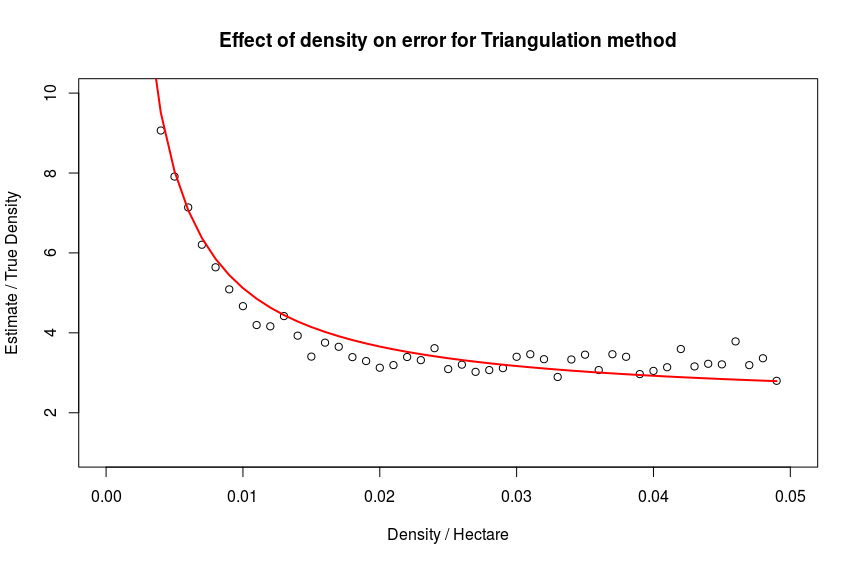
\includegraphics[width = 0.9\textwidth, center]{/home/stuart/Dropbox/academic/phd/gibbons/gibbon_simulation/plots/strauss_hardcore/error-density.png}
\caption{\emph{Effect of population density on estimation error ($\sigma = 500$).}}
\label{error-density}
\end{figure}

In figure \ref{error-sigma} we consider how the error is influenced by the detectability parameter $\sigma$. It can be seen that for realistic levels of $\sigma$ ($400 \leq \sigma \leq 1000$) there is a strong negative correlation between $\sigma$ and bias. However, this then quite rapidly stabilises. The graph illustrates the importance of maximising $\sigma$ in real instances. In particular, it supports the need for surveys to occur over multiple days, since each additional day will typically increase the true value of $\sigma$ (as it increases the chance of detection at plausible distances). In addition, surveying over multiple days could change the shape of the detection function - for example a Hazard rate model may be more accurate.\\

\begin{figure}[h]
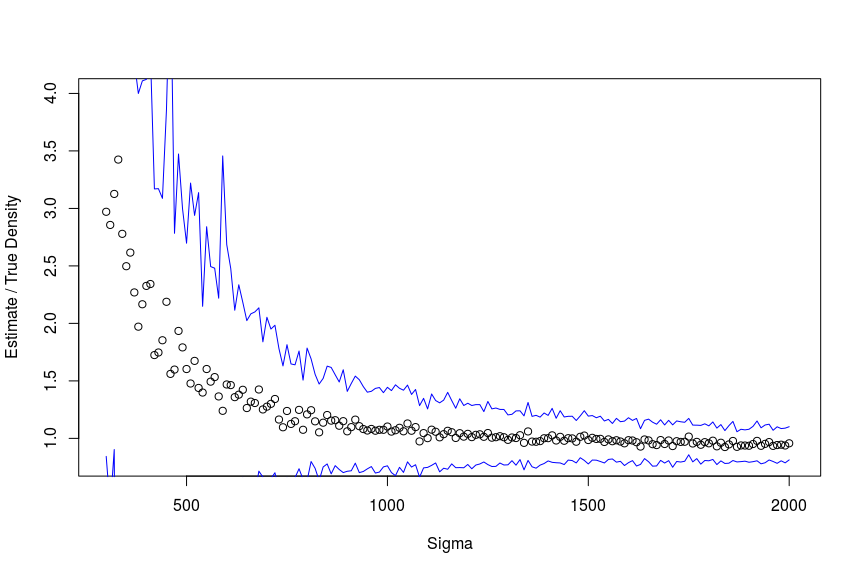
\includegraphics[width = 0.9\textwidth, center]{/home/stuart/Dropbox/academic/phd/gibbons/gibbon_simulation/plots/strauss_hardcore/error-sigma.png}
\caption{\emph{Effect of $\sigma$ on density estimation error (density $2km^{-2}$).}}
\label{error-sigma}
\end{figure}

We conjecture a number of methodologial reasons for the positive bias exhibited in these preliminary results. Primarily, we believe the estimated listening area is significantly underestimated by discarding the portions of each listeners individual effective listening area that does not overlap with others. This could be explained by the fact the effective listening area computed for each listener actually represents the area of `certain' detection by at least two listeners, since detections heard by one listener are previously discarded. Hence, reducing these areas even further via intersection causes under-estimation of effective area and thus positive bias in density estimates. If this issue is mitigated, perhaps by taking the union of the EDR areas for each post, then it will be important to include all detections heard by at least two listeners and not those only inside this union. This is essential due to the definition of the EDR, in particular, that the number of calls heard beyond the EDR is equal to the expected number missed below.\\

%Evidence for this argument is found in figure \ref{error-density-union}, where positive bias is significantly reduced or eliminated by instead combining the estimated effective listening areas for each detector to compute the overall effective area.\\

There is also a potential for bias in the calculation of the effective distance radius. However, we conjectue in comparison to the above the effect of this would be minor. Bias could be caused by non-uniformity in detection probability at a given radial distance in the plane due to the fact groups detected by only one listener are discarded. That is, detection probability is not independent of bearing, as assumed. Thus, a fundamentally two-dimensional problem is being treated as one-dimensional by distance software. We are currently looking into whether or not the pooling robustness property of distance sampling estimators mitigates this issue.

%\begin{figure}[H]
%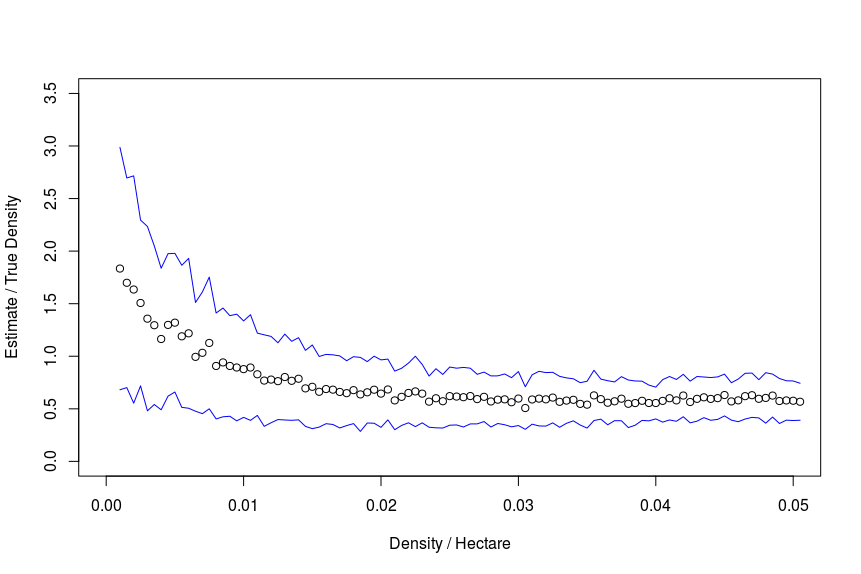
\includegraphics[width = 0.9\textwidth, center]{/home/stuart/Dropbox/academic/%phd/gibbons/gibbon_simulation/plots/strauss_hardcore/error-density-union.png}
%\caption{\emph{Effect of population density on estimation error with modified %triangulation method ($\sigma = 500$).}}
%\label{error-density-union}
%\end{figure}

\bibliographystyle{unsrt}
\bibliography{bibliography}
\end{document}
